
\chapter*{Wprowadzenie}
\addcontentsline{toc}{chapter}{Wprowdzenie}  
\markboth{Wprowadzenie}{Wprowadzenie}

Linie kolejowe dużych prędkości wciąż są aktualnym elementem procesu rozwoju transportu zarówno w Polsce jak i na świecie. Według International Union of Railways (UIC)  w ciągu ostatnich 10 lat globalna liczba pasażerokilometrów z wykorzystaniem kolei dużych prędkości powiększyła się z ok 250 mld pkm/rok do ponad 1000 mld pkm/rok \parencite{UIC2021}. Zdecydowana większość przyrostu wynika z gwałtownego wzrostu inwestycji w Koleje Dużych Prędkości (KDP) w Chinach. Europejskie kraje rozpoczęły eksploatację KDP już w latach 80' XX w. W Polsce z uwagi na warunki polityczne i gospodarcze skonkretyzowane plany budowy KDP zostały przyjęte dopiero w 2008 roku w dokumencie \parencite{UchwaaNr276}. W kolejnej dekadzie postawiono na modernizację istniejących linii kolejowych, w tym na dostosowanie linii nr 4 (CMK) i linii nr 9 do prędkości 200 km/h. W pracy \parencite{Towpik2010} opisano szczegółowo rozwój oraz zalety jakie przynosi Kolej Dużych Prędkości. 

\begin{figure}[hbt!]
	\centering
	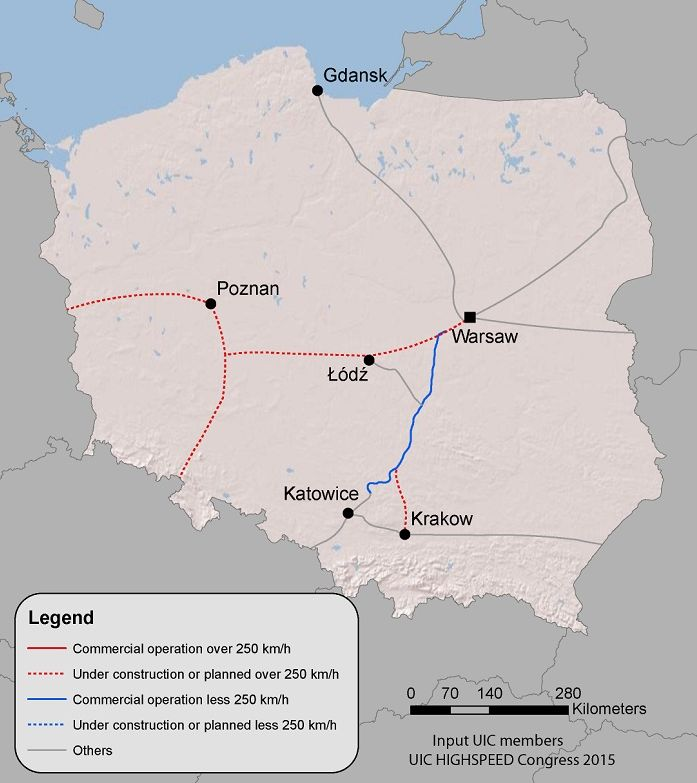
\includegraphics[width=0.7\linewidth]{/mosty_wstep/mapa.jpg}
	\captionsetup{justification=centering}
	\caption{Mapa planowanych i zrealizowanych linii kolejowych dużych prędkości w Polsce - UIC HIGH-SPEED Congress 2015 \parencite{UIC2015}}
	\label{fig:LDP_mapa}
\end{figure}

Pomimo upływu lat nie ulega wątpliwości, że sieć KDP jest kluczowym elementem rozwoju Państwa \parencite{Raczynski2010}. Pozwala zwiększyć atrakcyjność kolei względem pozostałych środków komunikacyjnych, zwiększa spójność państw wchodzących w sieć połączeń czy też podnosi atrakcyjność gospodarczo-społeczną. W 2017 roku przyjęto kolejną uchwałę mówiącej o rozbudowie Kolei Dużych Prędkości w Polsce w związku z budową Centralnego Portu Komunikacyjnego \parencite{UchwaaNr173}. 


Oczywiście budowa infrastruktury kolejowej ściśle wiąże się przekraczaniem przeszkód i budową obiektów inżynierskich. W przypadku KDP jadący tabor musi mieć zagwarantowane restrykcyjne warunki dotyczące bezpieczeństwa przejazdu i komfortu pasażerów. W konsekwencji, przy projektowaniu mostów związane jest to przede wszystkim z większym ograniczeniem przemieszczeń i przyspieszeń konstrukcji \parencite{Niemierko}. Z drugiej strony wciąż postępujący rozwój technologi, materiałów budowlanych i informatyzacja procesu projektowania sprawiają, że używane są coraz wytrzymalsze materiały w zoptymalizowanych strukturach. Dodatkowo rośnie także zapotrzebowanie na coraz większe, spektakularne konstrukcje pozwalające na przekroczenie dotychczas niepokonanych przeszkód. Sytuacja ta jest szczególnie widoczna w mostach łukowych, popularnych w ciągu tras kolejowych. Pozwalają one na pokonanie większych rozpiętości niż mosty belkowe, a jednocześnie są konkurencyjne cenowo dla mostów kratownicowych (wer.). Nie bez znaczenia, są również aspekty estetyczne. Odczucia obserwatora, a w tym również organów decydujących o budowie przeprawy, odnoszą się nie tylko do funkcji oraz finansów, ale także do krajobrazowego znaczenia mostu, aspektu kulturowego i filozoficznego. W przypadku mostów łukowych odczucia te są niezwykle silne \parencite{Kido_Cywiński_2019,Kido_Cywiński_2021}. Mosty łukowe z jednej strony naturalnie odnoszone są do pozytywnie odbieranej tęczy \parencite{Prandowski1994}, a z drugiej w miastach mogą stanowić swoistą bramę wjazdową będąc obiektem typu "landmark". W wyniku tych wszystkich czynników budowane konstrukcje są uatrakcyjniane wizualnie, są lżejsze i smuklejsze bądź posiadają nietypowe formy. Niestety, z reguły wpływa to na zwiększenie podatności na drgania konstrukcji. Na rysunku \ref{fig:bridges_arch_monatage} pokazano szkielet łukowego mostu drogowego \textit{Brandangersund bridge} o rozpiętości 220 m w trakcie montażu. Most ten uważany jest za najsmuklejszą konstrukcję łukową na świecie \parencite{Larssen2011}.

\begin{figure}[hbt!]
	\centering
	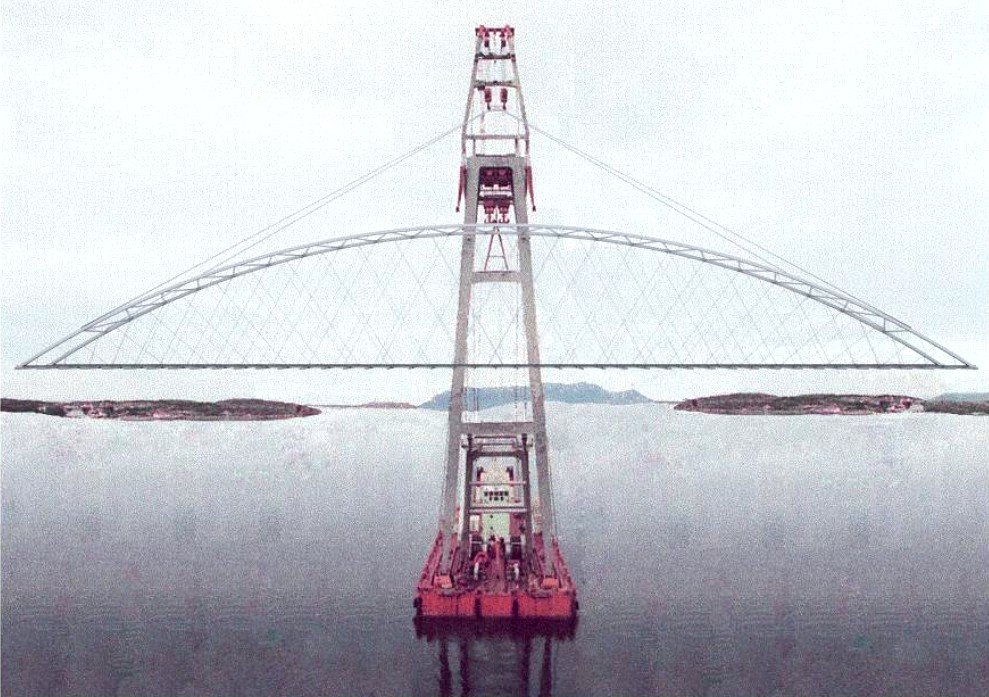
\includegraphics[width=0.7\linewidth]{/mosty_wstep/montaz_akvik_sound_bridge.jpg}
	\captionsetup{justification=centering}
	\caption{Montaż szkieletu mostu drogowego o dźwigarze łukowym i wieszakach typu Network (źródło: \parencite{Tveit2014})}
	\label{fig:bridges_arch_monatage}
\end{figure}

W tradycyjnym podejściu do projektowania mostów kolejowych historycznie największy nacisk stawiano na kwestię wytrzymałości ustroju wyrażoną stanem granicznym nośności z uwzględnieniem trwałości zmęczeniowej. Warunki użytkowe - stan graniczny użytkowania - ograniczały się do sprawdzenia największego ugięcia dźwigarów pod obciążeniem normowym \parencite{PKNf}. W stalowych mostach kolejowych zalecano również sprawdzenie okresu poprzecznych drgań własnych przęsła oraz kątów obrotów na podporach. Uwzględnienie naturalnie dynamicznego zjawiska przejazdu taboru po obiekcie ograniczone było jedynie do zastosowania współczynnika dynamicznego, zwiększającego efekty obciążeń statycznych i nieuwzględniającego efektów rezonansu. Brak katastrof i spektakularnych awarii mostów kolejowych pozwala stwierdzić, że narzucone normami warunki projektowania sprawdziły się w przypadku mostów kolejowych dla kolei poruszającej się z prędkościami poniżej 160 km/h. W nowszych normatywach, jakimi sa Eurokody, wyraźnie rozdzielono stan graniczny nośności od stanu granicznego zmęczenia, a także istotnie rozbudowano sprawdzenia stanu granicznego użytkowania oraz weryfikację zachowania dynamicznego przęsła. Działania te podjęto na podstawie wniosków i doświadczeń z pracy komitetów naukowych badających efekty przejazdów taboru po mostach. W dużej mierze prace te skupione były na przejazdach z prędkością do 350 km/h. Zidentyfikowano i opisano oddziaływania pionowe i poprzeczne występujące wskutek przejazdu. Obecnie w projektowaniu wymagane jest więc nie tylko by konstrukcja była nośna, ale również gwarantowała bezpieczeństwo i komfort użytkowania pasażerów. Narzuca to na barki projektanta szereg nowych obowiązkowych weryfikacji projektowanej konstrukcji. Dynamika typowych konstrukcji belkowych i płytowych przy przejeździe z dużą prędkością została bardzo dobrze rozpoznana i opisana za pomocą tablic i nomogramów. W pozostałych przypadkach wymagane są zaawansowane i czasochłonne testy numeryczne. 

Mostowe konstrukcje łukowe są bardzo różnorodne. Różnią się położeniem pomostu względem dźwigarów, dystrybucją materiału i sztywności między elementami konstrukcyjnymi czy układem elementów łączących dźwigar łukowy z pomostem. Bogactwo form sprawia, że trudno przewidzieć jaki zestaw parametrów będzie optymalny dla danego usytuowania przeprawy i warunków przejazdu. Wszak w poszukiwaniu najlepszego rozwiązania należy uwzględnić szereg wymienionych wyżej kwestii: nośność konstrukcji, trwałość, bezpieczeństwo, a aktualnie także również komfort dynamiczny przy przejeździe z dużą prędkością. Jednocześnie przy spełnieniu wszystkich obostrzeń rozwiązanie powinno być również możliwie tanie, aby jej wykonanie było opłacalne i miało szansę zaistnieć. Obecnie mnogość możliwości ukształtowania konstrukcji sprawia, że ostateczne rozwiązania zwykle są dalekie od optymalnych technicznie jak i finansowo. Poniższa praca ma za zadanie pomóc rozwiązać problem doboru parametrów konstrukcji łukowych konstrukcji kolejowych w kontekście przejazdów z duża prędkością.


\section*{Cel pracy}
Celem pracy jest określenie wpływu poszczególnych elementów konstrukcyjnych i wyznaczenie ich optymalnych parametrów dla stalowego, kolejowego mostu łukowego z jazdą dołem uwzględniając zachowanie dynamiczne obiektu przy przejeździe pociągów dużej prędkości.
W szczególności, działania wykonane na drodze do głównego rezultatu miały na celu:
\begin{itemize}
	\item zweryfikowanie skuteczności metod operacyjnej analizy modalnej przy identyfikacji modalnej stalowych, kolejowych obiektów łukowych średniej rozpiętości,
	\item opracowanie metodyki kalibracji modelu numerycznego mostu kolejowego za pomocą metod wielokryterialnej optymalizacji globalnej, z wykorzystaniem rezultatów identyfikacji modalnej i standardowych pomiarów prowadzonych w trakcie próbnych obciążeń mostów,
	\item opracowanie metodyki optymalizacji wielokryterialnej mostów kolejowych w ciągu Linii Dużych Prędkości (LDP) ze szczególnym uwzględnieniem dynamiki konstrukcji,
	\item ocenę wpływu poszczególnych parametrów konstrukcji mostu łukowego na zachowanie dynamiczne pod obciążeniem pociągami dużej prędkości.
\end{itemize}


\section*{Teza pracy}
Możliwe jest określenie wpływu wymiarów elementów konstrukcyjnych mostu łukowego na jego zachowanie dynamiczne i znalezienie optymalnego finansowo i dynamicznie rozwiązania dla obiektów w ciągu linii kolejowych dużych prędkości. Rezultaty optymalizacji mogą pozwolić określić zalecenia doboru parametrów konstrukcji łukowej zapewniające minimalny koszt budowy oraz dostateczną odporność dynamiczną mostu na liniach dużych prędkości.

\section*{Struktura pracy}
Praca składa się z wprowadzenia, pięciu rozdziałów, podsumowania oraz zestawienia bibliograficznego. 

W \textit{Rozdziale 1} przedstawiono wszystkie główne aspekty dotyczące charakterystyki i modelowania mostów łukowych oraz występujących na nich obciążeń dynamicznych. Początkowo przedstawiono charakterystykę i klasyfikację mostów łukowych ze szczególnym uwzględnieniem różnic w elementach konstrukcyjnych. W skróconej formie przedstawiono Metodę Elementów Skończonych oraz sposoby kalibracji modelu numerycznego. Na koniec omówiono oddziaływania dynamiczne występujące na mostach kolejowych oraz obowiązujące normatywy w zakresie projektowania tychże mostów. Do każdej z części zaprezentowano obszerny przegląd literatury przedmiotu.

\textit{Rozdział 2} zawiera zbiór podstawowych informacji na temat dynamicznej analizy konstrukcji. Przedstawiono metody analizy modalnej, jako grupy metod wyznaczania parametrów dynamicznych konstrukcji. W syntetyczny sposób pokazano rozwiązanie problemu własnego dynamiki czyli teoretycznej analizy modalnej. Przedstawiono w uporządkowany sposób istniejące metody wyznaczania odpowiedzi układu drgającego, zarówno o jednym jak i wielu stopniach swobody. Opisano także miary i modele opisujące efekty tłumienia drgań konstrukcji. W każdym z fragmentów zwrócono szczególną uwagę na elementy istotne z punktu widzenia dalszych prac: identyfikacji modalnej rzeczywistej konstrukcji i analizy dynamicznej modelu numerycznego przy poruszającym się obciążeniu.

\textit{Rozdział 3} stanowi opis jednej z rodzin metod identyfikacji modalnej - Operacyjnej Analizy Modalnej (OMA). Początkowo przedstawiono koncepcję oraz przytoczono podział i klasyfikację istniejących algorytmów OMA. Zawarto również przegląd literatury mówiącej o zastosowaniach OMA w praktyce inżynierskiej. Do identyfikacji wybranego obiektu badawczego wykorzystano metodę NExT-ERA. Dokonano jej szczegółowego opisu syntetycznego oraz omówiono właściwości metody. Następnie przedstawiono opis stworzonej aplikacji komputerowej do identyfikacji modalnej bazującej na algorytmie NExT-ERA. Zaprezentowano metody obróbki i łączenia sygnałów, dobór parametrów metody i sposoby oceny poprawności rozwiązania. Wykonano test numeryczny oraz laboratoryjny samej metody, jak i stworzonej aplikacji komputerowej.

\textit{Rozdział 4} zawiera przedstawienie zagadnienia optymalizacji konstrukcji ze szczególnym uwzględnieniem nowoczesnych metod numerycznych. Wstępnie omówiono i sklasyfikowano metody optymalizacji w kontekście projektowania konstrukcji. Do dalszych analiz wybrano metodę poszukiwania minimum globalnego algorytmem metaheurystycznym Particle Swarm Optimization (PSO). Opisano metodę oraz dobrane parametry sterujące algorytmem: wielkość roju, warunki brzegowe i topologię roju. Przedstawiono zastosowania algorytmu przy rozwiązywaniu problemów inżynierskich występujące w literaturze. Wykonano przykład teoretyczny metody z jedną funkcją celu. Następnie opisano uogólnienie metody jednokryterialnej do wielokryterialnej z zastosowaniem operatora dominacji w sensie Pareto. Dla wariantu o kilku funkcjach celu również wykonano przykład testowy.

\textit{Rozdział 5} jest syntezą wszystkich wcześniej wykonanych prac. Zaprezentowano w nim kompleksową analizę mającą na celu optymalizację konstrukcji istniejącego wiaduktu WK-2 w ciągu Pomorskiej Kolei Metropolitalnej w Gdańsku. Analiza składała się z trzech głównych etapów. Pierwszym była identyfikacja modalna konstrukcji metodą OMA w celu określenia rzeczywistych parametrów modalnych. Następnie przedstawiono procedurę kalibracji modelu numerycznego z zastosowaniem wyników identyfikacji modalnej i badań pod próbnym obciążeniem. Kolejno opisano przeprowadzoną na przygotowanym modelu numerycznym wariantową optymalizację wielokryterialną algorytmem PSO. Przedstawiono rezultaty i wyciągnięto wnioski.

Na końcu rozprawy znajduje się \textit{Podsumowanie}. Ujęto w nim główne wnioski wynikające z wszystkich przeprowadzonych prac oraz określono kierunki dalszej pracy nad wykorzystaniem identyfikacji modalnej i optymalizacji w analizie konstrukcji mostowych.





